\documentclass[10pt,a4paper,final]{report}
\usepackage[utf8]{inputenc}
\usepackage[english]{babel}
\usepackage{amsmath}
\usepackage{amsfonts}
\usepackage{amssymb}
\usepackage{float}
\usepackage{fancyhdr}
\usepackage{enumitem}
\usepackage{graphicx}
\pagestyle{fancy}

\title{Selfstudy 3 - Database}
\author{sw608f14 - Daniel S. F., Lars A., Mathias W. P. and Søren S. A.}

\begin{document}

\maketitle

\section*{1. ER Modeling}
\begin{figure}[H]
     \centering
     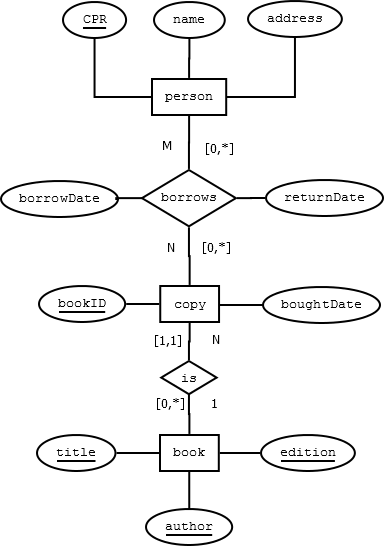
\includegraphics[scale=0.5]{exercise1}
     \caption{ER Diagram - Exercise 1}
\end{figure}

\section*{2. Banking System}

\begin{description}[style=nextline]
     \item[phone]
     $\{[\underline{number}, provider, contract]\}$
     \item[has           ]
     $\{[\underline{number \rightarrow phone, SSN \rightarrow customer}]\}$
     \item[customer]
     $\{[\underline{SSN}, name, address]\}$
     \item[account]
     $\{[\underline{accountNumber}, type, balance, owner \rightarrow customer]\}$
     \item[statement]
     $\{[\underline{ID, accountNumber \rightarrow account}, date]\}$
\end{description}


\section*{3. Relational Algebra}
\subsection*{1.}
\subsubsection*{$\pi_{species, zooID} (animals)$}
\begin{tabular}{|c|c|}
\hline 
species & zooID \\ 
\hline 
giraffe & 1 \\ 
\hline 
giraffe & 2 \\ 
\hline 
giraffe & 3 \\ 
\hline 
ape & 1 \\ 
\hline 
ape & 2 \\ 
\hline 
owl & 2 \\ 
\hline 
owl & 1 \\ 
\hline 
\end{tabular} 

\subsubsection*{$\sigma_{country='Germany'}(zoos)$}
\begin{tabular}{|c|c|c|c|}
\hline 
zooID & name & city & country \\ 
\hline 
1 & Zoo Frankfurt & Frankfurt & Germany \\ 
\hline 
\end{tabular} 

\subsubsection*{$\pi_{zooID}(\sigma_{country='Germany'}(zoos))$}
\begin{tabular}{|c|}
\hline 
zooID \\ 
\hline 
1 \\ 
\hline
\end{tabular}

\subsubsection*{$(\pi_{species, zooID} (animals)) \div (\pi_{zooID}(\sigma_{country='Germany'}(zoos)))$}

\begin{tabular}{|c|c|}
\hline 
species & zooID \\ 
\hline  
giraffe & 2 \\ 
\hline 
giraffe & 3 \\
\hline 
ape & 2 \\ 
\hline 
owl & 2 \\
\hline 
\end{tabular}

\subsection*{2.}
\subsubsection*{$(\rho_{T1}(animals)) \Join_{T1.zooID = T2.zooID} (\rho_{T2}(animals))$}
\begin{tabular}{|c|c|c|c|c|c|c|c|c|c|c|c|c|c|}
\hline 
T1.animalID & T1.nickname & T1.species & T1.gender & T1.zooID & T1.father & T1.mother & T2.animalID & T2.nickname & T2.species & T2.gender & T2.zooID & T2.father & T2.mother \\ 
\hline 
1 & Tally & giraffe & female & 1 & 3 & 2 & 1 & Tally & giraffe & female & 1 & 3 & 2 \\ 
\hline 
1 & Tally & giraffe & female & 1 & 3 & 2 & 4 & Stan & ape & male & 1 & 5 & - \\ 
\hline 
1 & Tally & giraffe & female & 1 & 3 & 2 & 7 & Jahoo & owl & male & 1 & 10 & 11 \\ 
\hline 
1 & Tally & giraffe & female & 1 & 3 & 2 & 8 & Boo & owl & female & 1 & 10 & 11 \\ 
\hline 
1 & Tally & giraffe & female & 1 & 3 & 2 & 10 & Huhuu & owl & male & 1 & - & - \\ 
\hline 
1 & Tally & giraffe & female & 1 & 3 & 2 & 11 & Eule & owl & female & 1 & - & - \\ 
\hline 
2 & Kathy & giraffe & female & 2 & - & - & 5 & Pam & ape & male & 2 & - & - \\ 
\hline 
2 & Kathy & giraffe & female & 2 & - & - & 6 & Uhu & owl & male & 2 & 9 & 8 \\ 
\hline 
... & • & • & • & • & • & • & • & • & • & • & • & • & • \\ 
\hline 
\end{tabular} 
Was too big. Going straight to result:

\subsubsection*{$\pi_{T1.nickname} ( \sigma_{T1.animalID = T2.father \lor T1.animalID = T2.mother}((\rho_{T1}(animals)) \Join_{T1.zooID = T2.zooID} (\rho_{T2}(animals))))$}
\begin{tabular}{|c|}
\hline 
T1.Nickname \\ 
\hline 
Wohoo \\ 
\hline 
Huhuu \\ 
\hline 
Eule \\ 
\hline 
\end{tabular} 

\section*{4. Relational Calculus}
\subsection*{1.}
$$\pi_{sname}((Suppliers) \Join ((\sigma_{color='red'}(Parts)) \Join (Catalog)))$$

$$\{<s.sname>|s \in Suppliers \land \exists c(c \in Catalog \land c.sid = s.sid \land \exists p (p \in Parts \land p.pid = c.pid \land p.color = 'red'))\}$$

$$\{<sname>| <sid,sname,\_> \in Suppliers \land <sid,pid,\_> \in Catalog \land <pid,\_,'red'> \in Parts\}$$

\subsection*{2.}
$$\pi_{sid}((\sigma_{color='red' \lor color = 'green'}(Parts)) \Join (Catalog))$$

$$\{<c.sid>|c \in Catalog \land \exists p ( p \in Parts \land p.pid = c.pid \land (p.color = 'red' \lor p.color = 'green'))\}$$

$$\{<sid>| <sid,pid,\_> \in Catalog \land (<pid, \_, 'red'> \in Parts \lor <pid,\_, 'green'> \in Parts)\}$$
\subsection*{3.}
$$\pi_{sid}((Catalog)\Join((\rho_{T1}(\sigma_{color = 'red'}(Parts)))\Join_{T1.pid = T2.pid}(\rho_{T2}(\sigma_{color = 
'green'}(Parts)))))$$

$\{<c.sid>| c \in Catalog \land \exists p1 (p1 \in Parts \land p1.color = 'red'  \land c.pid = p1.pid \land \exists c1 (c1 \in Catalog \land c1.sid = c.sid \land \exists p2 (p2 \in Parts \land p2.pid = c1.pid \land p2.color = 'green')))\}$

$$\{<sid>| <sid,pid,\_> \in Catalog \land (<pid, \_, 'red'> \in Parts \land <sid,pid',\_> \in Catalog \land <pid',\_,'green'> \in Parts)\}$$

\subsection*{4.}
$$\pi_{T1.sid, T2.sid}(\sigma_{T1.cost > T2.cost}((\rho_{T1}(Catalog))\Join_{T1.pid = T2.pid}(\rho_{T2}(Catalog))))$$

$$\{<c1.sid, c2.sid> | c1 \in Catalog \land c2 \in Catalog \land c1.pid = c2.pid \land c1.cost > c2.cost\}$$

$$\{ <sid1, sid2>| <sid1,pid,cost1> \in Catalog \land <sid2,pid,cost2> \in Catalog \land cost1 > cost2\}$$

\subsection*{5.}

$$\pi_{T1.pid}((\rho_{T1}(Catalog))\Join_{T1.pid = T2.pid \land T1.sid \neq T2.sid}(\rho_{T2}(Catalog)))$$

$$\{ <c.pid>| c \in Catalog \land \exists c2 (c2 \in Catalog \land c.pid = c2.pid \land c.sid \neq c2.sid)\}$$

$$\{<pid>|<sid1,pid,\_> \in Catalog \land <sid2,pid,\_> \land sid1 \neq sid2\}$$

\section*{5. Functional dependencies}
\begin{tabular}{|c|c|}
\hline 
FD & OK or violated? \\ 
\hline 
$A\rightarrow C$ & violated: tuples 3,4 \\ 
\hline 
$B\rightarrow A$ & OK \\ 
\hline 
 $C\rightarrow A$ & violated: tuples 1,3 \\ 
\hline 
$A\rightarrow B$ & violated: tuples 1,2 \\ 
\hline 
$B\rightarrow C$ & violated: tuples 3,4 \\ 
\hline 
$BC\rightarrow A$ & OK \\ 
\hline 
$AC\rightarrow B$ & OK \\ 
\hline 
\end{tabular} 
\end{document}